\documentclass{article}
\usepackage{graphicx,fancyhdr,amsmath,amssymb,amsthm,subfig,url,hyperref}
\usepackage[margin=1in]{geometry}
\usepackage{enumerate}
% \usepackage{algorithms}
\usepackage{bookmark}
\usepackage{tikz}
% \usetikzlibrary{arrows}
\usetikzlibrary{arrows.meta}
\usetikzlibrary{quotes}
\usepackage{extarrows}
\usepackage{clrscode3e}
\usepackage{float}
\usepackage{indentfirst}

%----------------------- Macros and Definitions --------------------------

%%% FILL THIS OUT
\newcommand{\studentname}{Jiang Caiwen}
\newcommand{\suid}{2019233157}
\newcommand{\exerciseset}{Homework 4}
\newcommand{\floor}[1]{\left\lfloor #1 \right\rfloor}
\newcommand{\ra}{\rightarrow}
\def\o{\ensuremath\varnothing}
%%% END



\renewcommand{\theenumi}{\bf \Alph{enumi}}

%\theoremstyle{plain}
%\newtheorem{theorem}{Theorem}
%\newtheorem{lemma}[theorem]{Lemma}

\fancypagestyle{plain}{}
\pagestyle{fancy}
\fancyhf{}
\fancyhead[R]{\sffamily\bfseries ShanghaiTech University}
\fancyhead[L]{\sffamily\bfseries CS240 Algorithm Design and Analysis}
\fancyfoot[L]{\sffamily\bfseries\studentname: jiangcw@shanghaitech.edu.cn}
\fancyfoot[R]{\sffamily\bfseries\thepage}
\renewcommand{\headrulewidth}{1pt}
\renewcommand{\footrulewidth}{1pt}

\graphicspath{{figures/}}

%-------------------------------- Title ----------------------------------

\title{CS240 \exerciseset}
\author{\studentname \qquad Student ID: \suid}

%--------------------------------- Text ----------------------------------

\begin{document}
\maketitle

\section*{Problem 1}
\quad\\
As before, all G are multigraphs.\\
Fix a min-cut C in the original multigraph G. By the same analysis as in the case of f, we have\\
	\begin{equation}
	\begin{aligned}
	&Pr[\text{C survives all contractions in f(G,t)}] \\
	&=\prod_{i=1}^{n-t}Pr[\text{C survives the i-th contraction}| \text{C survives the first (i-1)-th contraction}]\\
	&\ge \prod_{i=1}^{n-t}(1 - \frac{2}{n-i+1})            \\
	& = \prod_{k =t+1}^{n} \frac{k-2}{k}\\
	&= \frac{t(t-1)}{n(n-1)}\nonumber
	\end{aligned}
	\end{equation}
When $t = [1+n/\sqrt{2}]$, this probability is at least 1/2. The choice of t is due to our purpose to make this probability at least 1/2. You will see this is crucial in the following analysis of accuracy.\\
We denote by A and B the following eventd:\\
A: C survives all contractions in f(G,t);\\
B : size of min-cut is unchanged after  f(G,t);\\
Clearly,  A implies B and by above analysis $Pr[B] \ge Pr[A] \ge  \frac{1}{2}$\\
We denote by $p(n)$ the lower bound on the probability that randomized algorithm succeeds for a multigraph of n 
vertices, that is \\
$$ p(n) = \min\limits_{G:|V|=n}Pr[\text{randomized algorithm returns a min-cut in G}] $$
Suppose that G is the multigraph that achieves the minimum in above definition. The following recurrence holds for $p(n)$:\\
	\begin{equation}
	\begin{aligned}	
	p(n)&=Pr[\text{randomized algorithm returns a min-cut in G}]\\
	      &= Pr[\text{a min-cut of G is returned by }  cut2(G_1) \text{ or } cut2(G_2)]\\
	      &\ge 1- (1- Pr[B\cup  cut2(G_1) \text{ return a min-cut in } G_1])^2\\
	      &\ge 1- (1- Pr[A\cup  cut2(G_1) \text{ return a min-cut in } G_1])^2\\
	      & = 1- (1- Pr[A]Pr[ cut2(G_1) \text{ return a min-cut in } G_1|A])^2\\
	      & \ge 1 - (1- \frac{1}{2}p([1+n/\sqrt{2}]))^2\nonumber
	\end{aligned}
	\end{equation}
where A and B are defined as above such that $Pr[A]\ge 1/2$\\
The base case is that $p(n )= 1 $ for $n\le 6$.  By induction it is easy to prove that\\
$$p(n) = \Omega(\frac{1}{logn})$$
\\
\\	
\section*{Problem 2}
\quad\\
1. Let G  be a graph, and let $C_1,...C_r$ denote all its global min-cut, let $E_i$ denote the event that $C_i$  is returned by the Contraction Algorithm, let $E = \sum_{i=1}^{r}E_i$denote the event that the algorithm returns any global min-cut.\\
We know the contraction algorithm returns a min-cut with $prob \ge 2/n^2$, so\\
$$Pr[E] \ge 2/n(n-1)$$
$$Pr[E_i] \ge 2/n(n-1)$$
Then we have \\
$$Pr[E] = Pr[\sum_{i=1}^{r}E_i] = \sum_{i=1}^{r}Pr[E_i] \ge r \frac{2}{n(n-1)}$$ 
But clearly $Pr[E] \le 1$, and so we must have $r\le \frac{n(n-1)}{2}$.\\
\\
\\
2. The probability that the algorithm finds the minimum cut in G is at least $2/n^2$.\\
\begin{figure}[H]

	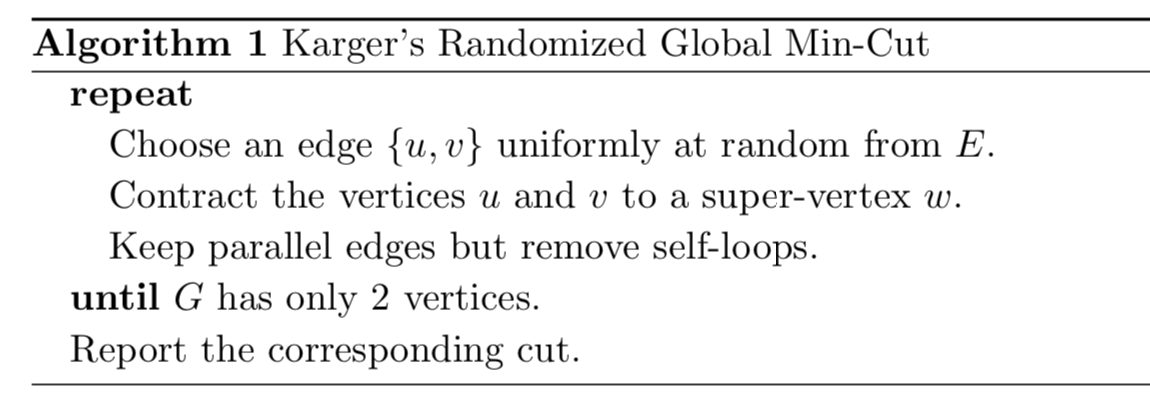
\includegraphics[width=0.7\textwidth]{1.png}
	
\end{figure}
Now we have to prove the correctness of the algorithm:\\
The probability of finding a min-cut seems low at face value, and goes to zero as $n \rightarrow \infty$. However, if we run the algorithm t times and output the smallest min-cut found over all runs, the probability of success
will be at least\\
$$1- (1- \frac{2}{n^2})^t$$
So if we set $t = cn^2$ for some constant c, the probability of failure will be at most $(1- \frac{2}{n^2})^{cn^2}\le e^{-2c}$. Thus to ensure the probability of failure is smaller than some fixed constant $\epsilon$, it is only necessary to run the algorithm $\frac{1}{2}log(\frac{1}{\epsilon})n^2$ times.\\
\\
\\
\section*{Problem 3}
\quad\\
Flip a coin, and set each variable true with probability 1/2, independently for each variable.\\
\rule[5pt]{10cm}{0.1em}\\
Appro-Max3SAT\\
\rule[5pt]{10cm}{0.05em}\\
 \indent    for i = 1 to n\\

\indent \indent 			 do Flip a fair coin \\

\indent \indent \indent 		 if Heads\\

	\indent \indent \indent \indent 			 then $x_i \leftarrow 1$\\
	\indent \indent \indent \indent 		  esle $x_i \leftarrow 0$\\

	\indent return x\\
	\rule[5pt]{10cm}{0.05em}\\	
 The running time of Approx-Max3SAT is O(n)\\
 Approx-Max3SAT is 7/8-approximate.\\
 Proof:\\
 Define the random variable:\\
 \begin{equation}
 Z_j = \left\{ 
 \begin{array}{ll}
 1, \text{if clause } C_j \text{ is satisfied}\\
 0 ,otherwise&\\
 \end{array}\right.
 \end{equation}
 Then, $Z= \sum_{j=1}^{k}Z_j$  is the number of clauses satisfied.\\
 The expected number of clauses satisfied is\\
 $$ E[Z] = \sum_{j=1}^{k}E[Z_j] = \sum_{j=1}^{k}Pr(C_j \text{is satisfied}) = \frac{7}{8}k$$
 because a random variable is at least its expectation some of the time, so we can get\\
 For any instance of 3-SAT, there exists a truth assignment that satisfies at least 7/8 of the clauses.\\
 
 
 \section*{Problem 4}
 The number of dice is represented by the H and T combinations of coins\\
 $$ HTH \rightarrow 1$$
 $$ HTT \rightarrow 2$$
 $$ THH \rightarrow 3$$
 $$ THT \rightarrow 4$$
 $$ TTH \rightarrow 5$$
 $$ TTT \rightarrow 6$$
 $$ HHH \rightarrow Null$$
 $$ HHT \rightarrow Null$$
We have a 3/4 chance of being able to get one of the 6 good results (HTH, HTT, THH, THT, TTH, TTT) that yields a random number from 1 to 6, and a 1/4 chance of having to reflip the coins (HHH or HHT). The key is that for those two results to be discarded, we only needed to flip 2 coins to determine that!\\
Let  X is the number of coins required\\
$$E[X] = 3/4 \times 3 +1/4 \times(2+E[X])$$
So, $E[X] = 11/3$\\
\\
\\

 \section*{Problem 5}
 For every array element $α$ and for every recursion level $t$, let $X_α,t$ be the indicator random variable for the event of choosing a bad pivot in $α’s$ subarray at level t:\\
 \begin{equation}
 X_{\alpha,t} = \left\{ 
 \begin{array}{ll}
 1, \text{iif, at level t, quicksort chose a bad pivot for the subarray containing } \alpha\\
 0 ,otherwise&\\
 \end{array}\right.
 \end{equation}
 
 fix $\alpha$ and take $T =c·logn$ for  constant $c,\delta$  to be chosen. We apply a Chernoff bound and simplify the exponential:\\
 	\begin{equation}
 	\begin{aligned}	
 	&Pr[\sum\limits_{i=1}^{T}X_{\alpha,i}\ge (1+\delta)E[  \sum\limits_{i=1}^{T}X_{\alpha,i}]]\\
 	&\le e^{-\delta^2 E[  \sum\limits_{i=1}^{T}X_{\alpha,i}]/2}\\
    &= e^{-\delta^2 \sum\limits_{i=1}^{T}E[  X_{\alpha,i}]/2}\\
 	& \le e^{-\delta^2T/2}\\
 	&= n^{-\delta^2c}\nonumber
 	\end{aligned}
 	\end{equation}
 Taking $\delta = 1$, we have\\
 $$Pr[\sum\limits_{i=1}^{T}X_{\alpha,i}\ge 2E[  \sum\limits_{i=1}^{T}X_{\alpha,i}]]\le \frac{1}{n^c}$$
 Thus we can get \\
 $Pr[\text{Runtime of quicksort}< nlongn]\le 1- \frac{1}{n^c}$
\end{document}

